\chapter{原型系统的综合测试结果}
本章将参数调优的结果添加到原型系统,分别使用模拟行驶数据以及实际采集的浮动车轨迹数据进行了测试,观察目标车辆在一段完整的行驶轨迹中,面对复杂的车辆交互情况时信誉值的变化特征,同时具体分析原型系统的测试结果是否与算法设计目标相吻合。

\section{模拟数据测试结果}
本节测试依然使用田字格道路,整合位置验证与消息传播的模拟,在目标车辆行驶路径中设置了不同的车辆分布模式、交互成功率,观察在较长时间行驶、遇到不同情况时,系统是否能够及时地通过信誉值的变化反映出车辆当前的行驶状态。

实验中,目标车辆共行驶经过了8条模拟道路,其信誉变化在原型系统的浏览器端使用leaflet地图组件得到了可视化展示,如图~\ref{fig:simmap}所示;对应的具体信誉曲线如图~\ref{fig:simplot}所示。在地图中,红色、绿色的点共同构成了目标车辆的行驶轨迹,利用转换为Geohash的地理数据进行绘制;每个数据点具体的颜色代表了目标车辆行驶至该位置时的信誉值,红色(\#FF0000)代表信誉值为0,,绿色(\#00FF00)代表信誉值为100,在该范围内进行颜色的梯度渐变。

除此之外,邻近车辆与目标车辆的交互结果也被展示在地图中。为了保证目标车辆的轨迹和信誉变化能得到清晰的体现,在地图中仅标注邻近车辆与目标车辆距离最近时该车所处的位置;此时两车之间的距离即为前文提到的计算所采用的交互距离。车辆交互的结果同样用颜色来表示:交互成功(位置验证成功,或者消息评价在5分以上)的邻近车辆被标记为蓝色,交互失败的车辆被标记为紫色。

\begin{figure}
  \centering
  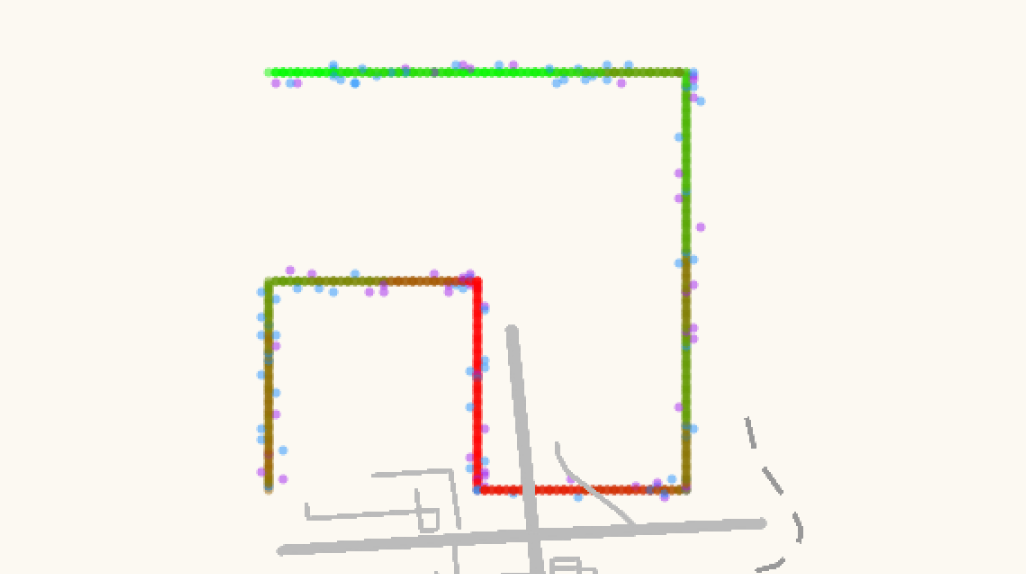
\includegraphics[width=0.8\linewidth]{figures/map4.png}
  \caption{模拟数据测试结果的地图展示}
  \label{fig:simmap}
\end{figure}

\begin{figure}
  \centering
  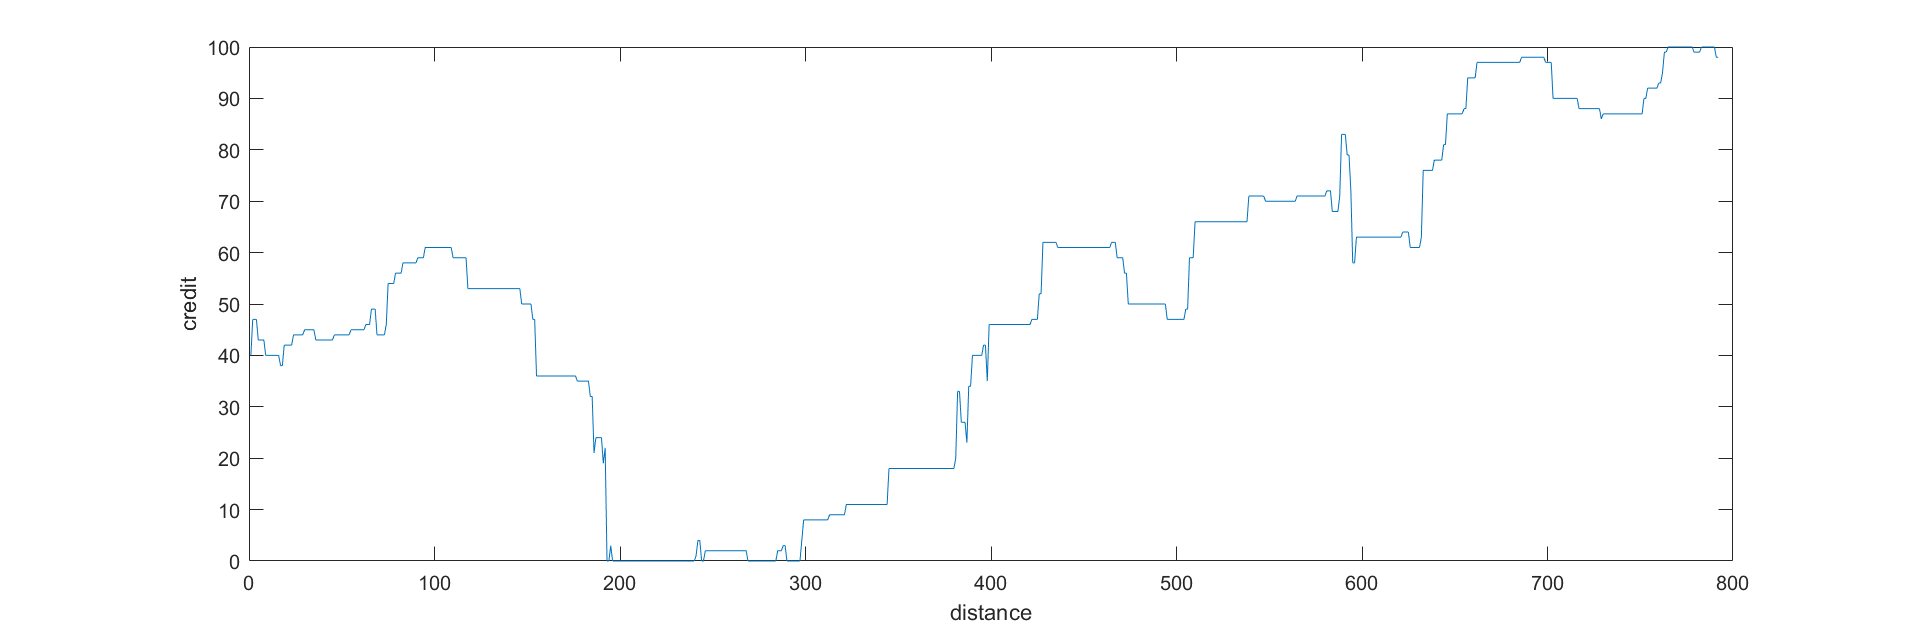
\includegraphics[width=1\linewidth]{figures/mapplot4.png}
  \caption{模拟数据测试结果的信誉曲线}
  \label{fig:simplot}
\end{figure}

\section{实际数据测试结果}

\subsection{数据处理}
本节中实验所用数据为2010年北京市浮动车轨迹数据,采集了1天之内北京市所有出租车的行驶记录,原始数据包括车辆ID、数据提交时间、车辆所在位置经纬度、车辆行驶状态(是否启动)等。实验依然选取了一辆车作为目标车辆,针对其特定的一段行驶记录进行信誉的计算。同时,根据该段行驶记录,从原始数据中筛选出在同一时刻与该目标车辆距离相近的其余浮动车作为邻近车辆,模拟车辆之间的交互。本节实验选取了一段包含696个数据点、总时长约为23分钟的浮动车行驶轨迹作为主要的测试对象,在行驶过程中与177台邻近车辆进行了交互。

\subsection{结果展示与分析}
目标车辆在地图中呈现的信誉可视化结果如图~\ref{fig:taximap}所示;对应的信誉曲线变化如图~\ref{fig:taxiplot}所示。与模拟数据的综合模拟测试结果相比,实际数据对应的信誉曲线变化相对更加平缓,基本不会出现由于少数几次交互结果导致信誉剧烈上升或下降的极端情况。其中的一部分原因是,实际数据在时间上的分布相对更加稀疏,目标车辆更新定位信息的平均时间间隔大约在2秒左右,而模拟数据测试中每两个数据点之间只间隔了1秒钟。

在实际数据的测试中,目标车辆的初始信誉值为40,行驶过程中在18-85分之间波动,数据波动最剧烈时在168秒内下跌了63分。

\begin{figure}
  \centering
  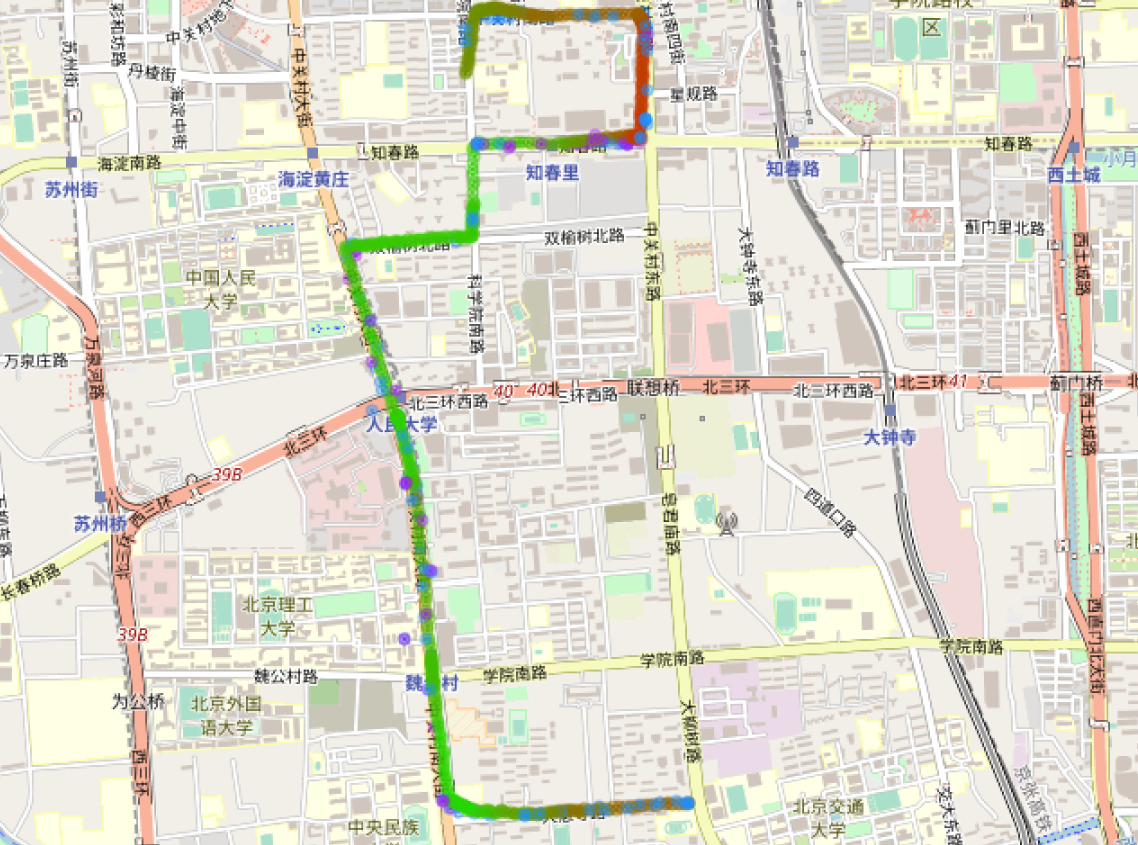
\includegraphics[width=0.8\linewidth]{figures/overview.png}
  \caption{实际数据测试结果的地图展示}
  \label{fig:taximap}
\end{figure}

\begin{figure}
  \centering
  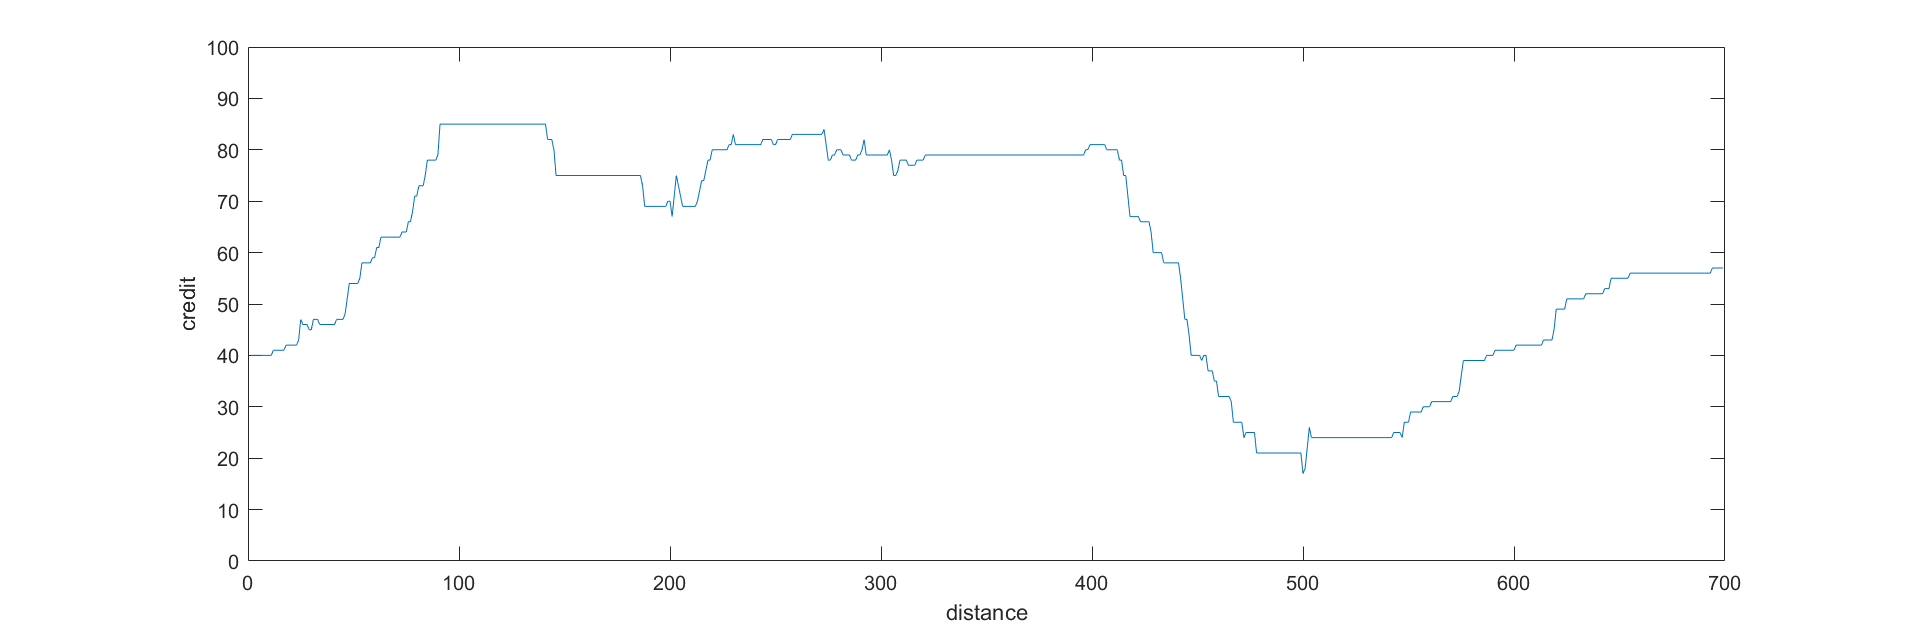
\includegraphics[width=1\linewidth]{figures/taxitest.png}
  \caption{实际数据测试结果的信誉曲线}
  \label{fig:taxiplot}
\end{figure}

图~\ref{fig:partials}展示了该段行驶路径在地图中放大后,交互结果及信誉变化的详细情况。图~\ref{fig:part1}中,目标车辆从从大柳树路与大慧寺路路口(近北京交通大学西门)出发,初始情况下默认信誉值为40,处于较低水平。在大慧寺路上行驶时,目标车辆稳定、持续地完成了多次成功的位置验证,使其信誉值逐步提升至较高水平;在右转处(约第150数据点左右)其定位信息产生了一定偏差,导致部分位置验证交互失败,但是由于其较高的历史正确率,信誉值仅产生了相对小幅度的下降。

随后目标车辆在中关村南大街上行驶,如图~\ref{fig:part2}所示,其中穿插有一定的交互失败情况,但是总体上依然有较高的交互成功率。结合图~\ref{fig:taxiplot},可以看到该段行驶过程中(约第200至第400数据点)信誉值仅有小幅波动,基本维持在同一水平(80分左右)。

图~\ref{fig:part3}中,目标车辆行驶至知春路中段时连续多次进行位置验证失败(约第400至第440数据点),其信誉水平已经明显下降。而从数据点在知春路路口的密集程度可以看出,目标车辆在知春路路口处进行了大约2-3分钟的等待。本节实验在该处进行了消息传播的模拟:目标车辆由于长时间等待向周围发送了路况拥堵的提示消息,但是实际上为正常的信号灯变动时间,因此该消息得到的负面评价会导致信誉值下降。由于路口处等待信号灯时车辆密度较大,该错误消息的传播导致其信誉值被大幅削减,从81分降低到18分的不可信水平。

此后目标车辆的轨迹如图~\ref{fig:part4}所示,可以看出目标车辆恢复了较高的交互成功率,在行驶过程中信誉值得到了缓慢但稳定的上升,最终在结束行驶时达到了57分。从最后两部分信誉值跌落与回升的趋势来看,失败的交互结果对于车辆信誉的惩罚是非常大的,想要进行弥补就必须要足够长的时间和足够好的交互结果,这使得部分恶意车辆难以通过个人或少数群体的操作骗取信誉,同时从整体上来看车辆的高信誉值也更加具有说服力。

\begin{figure}
  \centering
  \subcaptionbox{\label{fig:part1}}
    {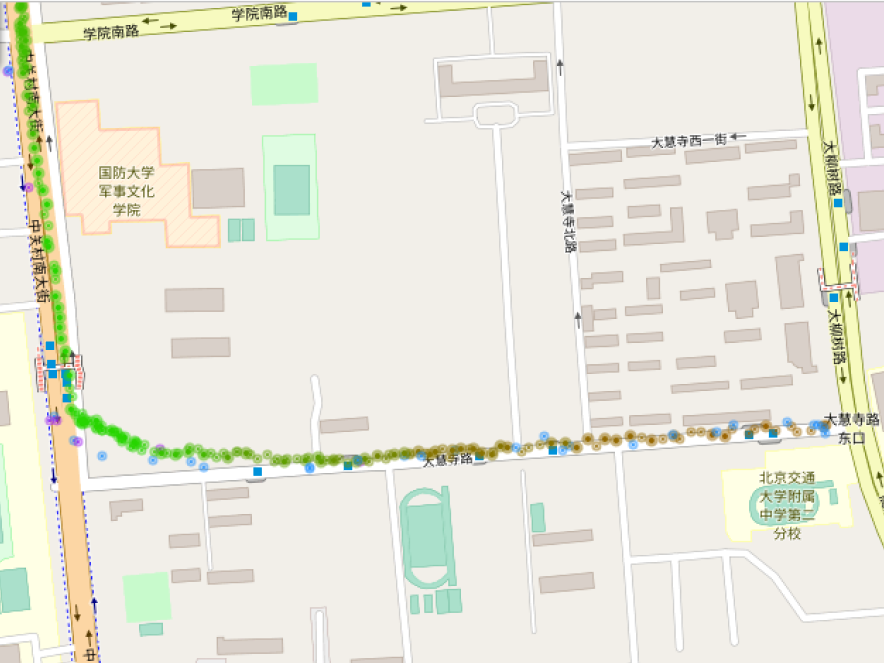
\includegraphics[width=0.49\linewidth]{figures/partial1.png}}
  \subcaptionbox{\label{fig:part2}}
    {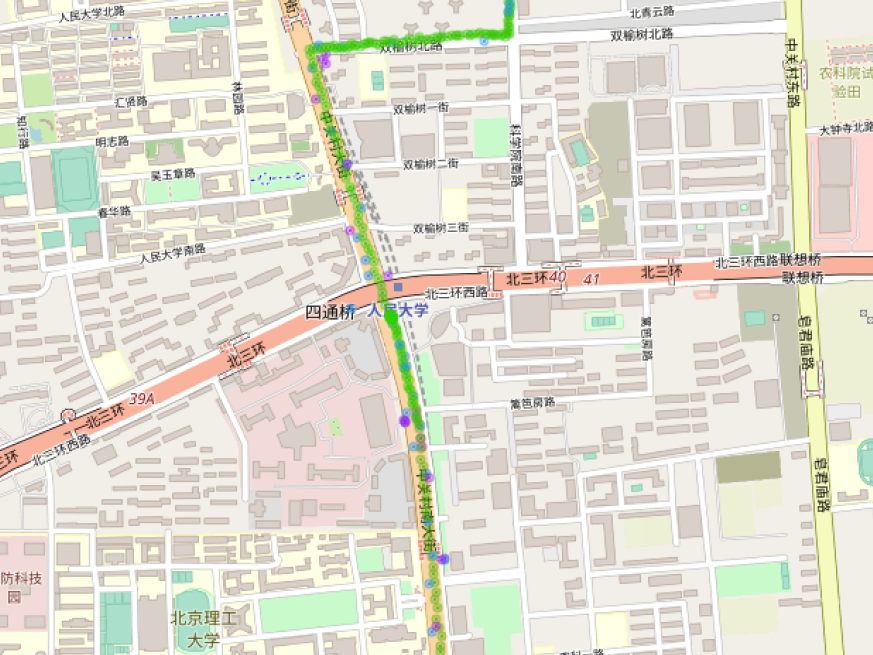
\includegraphics[width=0.49\linewidth]{figures/partial2.png}}
    \subcaptionbox{\label{fig:part3}}
    {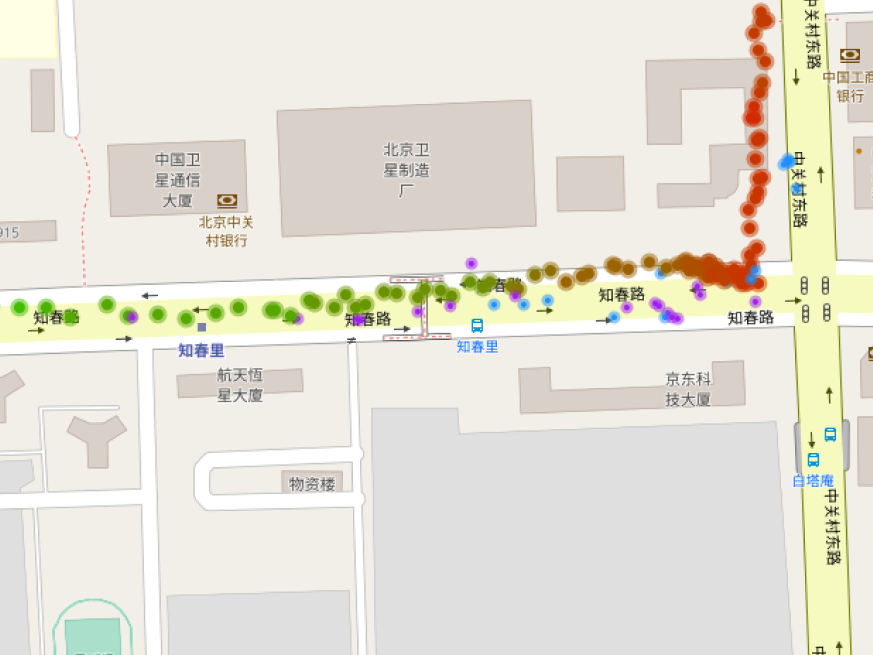
\includegraphics[width=0.49\linewidth]{figures/partial3.png}}
    \subcaptionbox{\label{fig:part4}}
    {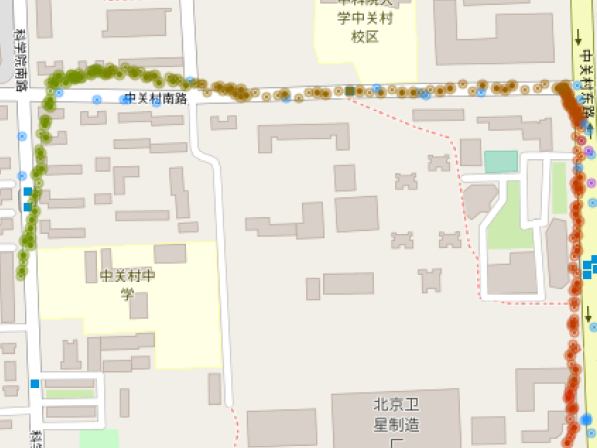
\includegraphics[width=0.49\linewidth]{figures/partial4.png}}
  \caption{实际数据测试结果的局部放大图}
  \label{fig:partials}
\end{figure}

\section{分析与改进}
从以上实验可以看出,本文提出的信誉算法在原型系统中得到了较好的体现,根据实时的车辆交互结果,能够相对迅速、灵敏地进行信誉值的调整,由该算法得到的车辆信誉在实际情况中能够较为合理、准确地体现该车辆在车载网中提供信息的可信度。由于条件限制,笔者不能使用更多的实际数据完善测试结果;可以将该系统扩展为面向多台车辆的应用,通过同时追踪多车的行驶动态及信誉变化,从整体交通状态的层面上对算法及原型系统进行更加全面的评估。

\section{本章小结}
本章利用模拟数据及真实浮动车数据对原型系统进行了综合测试,分析了车辆行驶过程中遇到的不同情况以及原型系统据此做出的信誉值调整。两种数据得到的测试结果均表明,该原型系统对于车辆活跃度展现出了较高的敏感度,相对于数据密度更大的模拟测试,实际数据测试得到的信誉曲线变化幅度更加缓和。
在系统中,车辆主要通过稳定、持续的成功友邻交互来得到信誉值的提升,并且完成该过程的难度要明显大于由失败交互结果导致的相同幅度的信誉值降低。同时,图~\ref{fig:part1}体现了位置验证历史成功率对信誉变化的平滑效果,图~\ref{fig:part3}体现了消息传播的评价分布对最终信誉变化的影响。通过对测试结果的具体讨论,可以认为该系统较好地完成了车辆信誉值评估的功能,其最终效果与算法理论设计中提出的目标较为符合。最后,本章提出了该算法及系统可能的改进和扩展方向。